% \chapter{Characterization at the electrode level}
\label{chap:graphite}

With the experience gained working on the projects described in the previous two sections, I was curious on the possibility of identify lithium plating in situ during reduction of the graphite though time-varying impedance. This is a huge topic, especially in the last years where company achieved (es. StoreDot) extreme fast charging. Fast charging, while enabiling a greater diffusion of electric veichles for the convience of it, should be use sparcelly. \colorbox{BurntOrange}{As described in the introduction}, chargin with high urrent densities pushes the potential of the negative electrode much lower than its themodynaic values to a point where lithium reduction is possible. Fast charging a battery every cycle inevitably reduced the life of the device. It is interesting though to know what happens after one fast charge cycle to the graphite electrode and if the impedance can retrive some information. The set-up used is similar to the one used for the project regarding silicon carbonitride and the mechanisms of sodium intercalation; I assemble a three electrode half cell in pouch format with natural graphite electrode and microscopic electrodeposited electrode, discharge the cell at 1C without any potential limitation but rather time limitation (i.e. charge) and then performed consecutive non-stationary impedance experiment in galvanostatic mode with increasing current density.

\section{Cell assembling}

For this project the working electrode was a graphite slurry of SBR and water doctor bladed on copper foil. The counter electrode was a square of lithium foil 22x22x?? mm (99.?? \%, Sigma Aldritch). An insulate copper wire current collector with diameter of 130um was produces with the same method described in the section before and the cell assemble using two glasfiber separator with the refernce copper wire between them, placed in such a way to have the exposed copper area in the center of the electrode area. 300 uL of electrolytic solution LiPF6 in EC:DMC 1M with 2\% of VC was poured in the cell and the device underwent 2 cycle of under-pressurization of 10 mbar to remove gasses from the pores while allowing the permeation of the liquid. The cell was sealed wit a coffe bag under a pressure of 10 mbar. \colorbox{Blue}{Transform in pascal}

\section{Time-varying impedance measurements}

\begin{figure}[H]
    \centering
    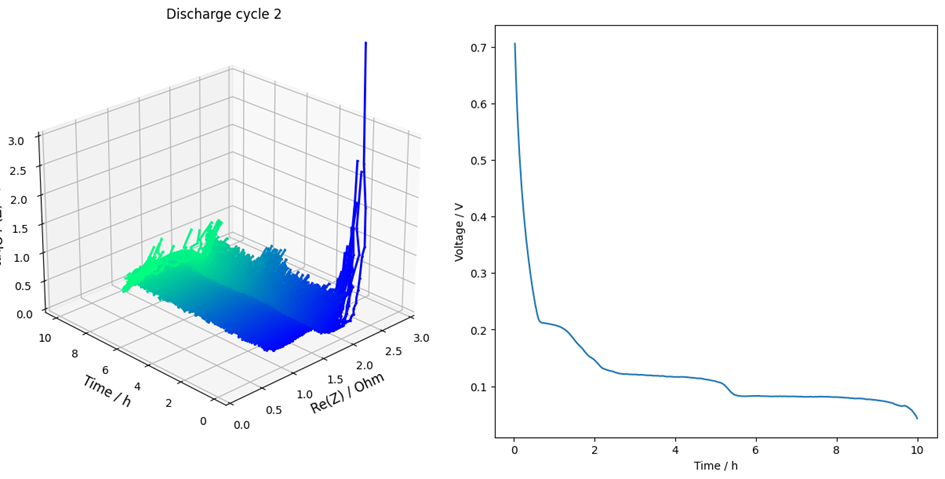
\includegraphics[width=\linewidth]{figures/application5/image1.png}
\end{figure}

\begin{figure}[H]
    \centering
    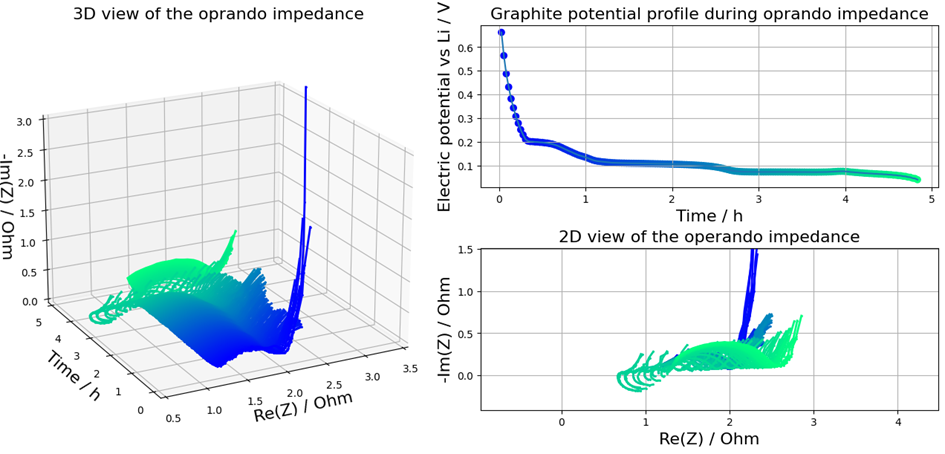
\includegraphics[width=\linewidth]{figures/application5/image2.png}
\end{figure}

\begin{figure}[H]
    \centering
    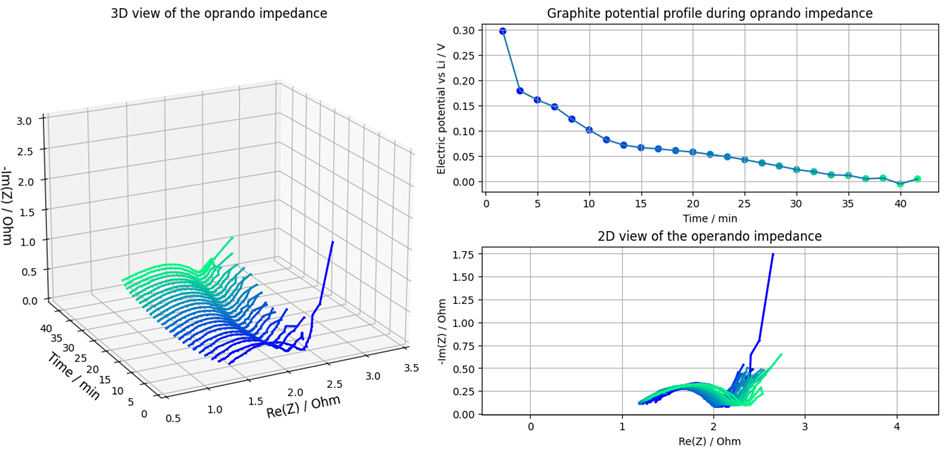
\includegraphics[width=\linewidth]{figures/application5/image3.png}
\end{figure}

\begin{figure}[H]
    \centering
    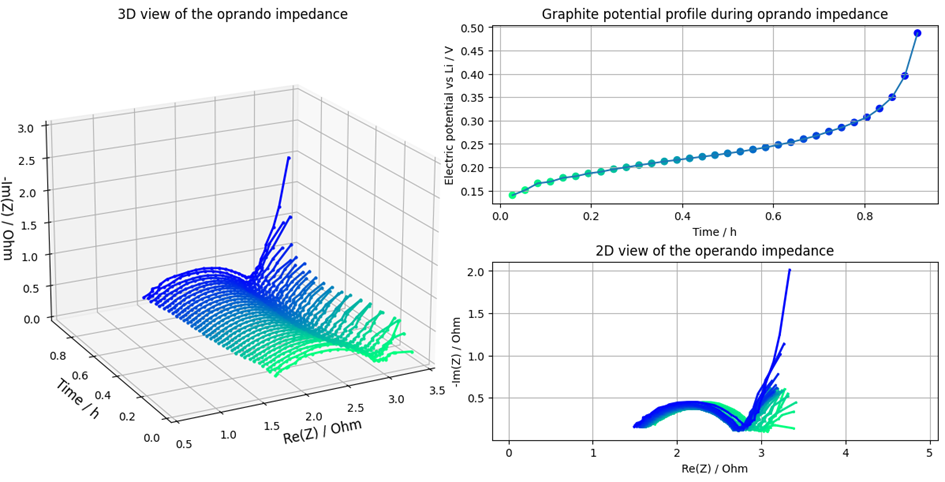
\includegraphics[width=\linewidth]{figures/application5/image4.png}
\end{figure}

\begin{figure}[H]
    \centering
    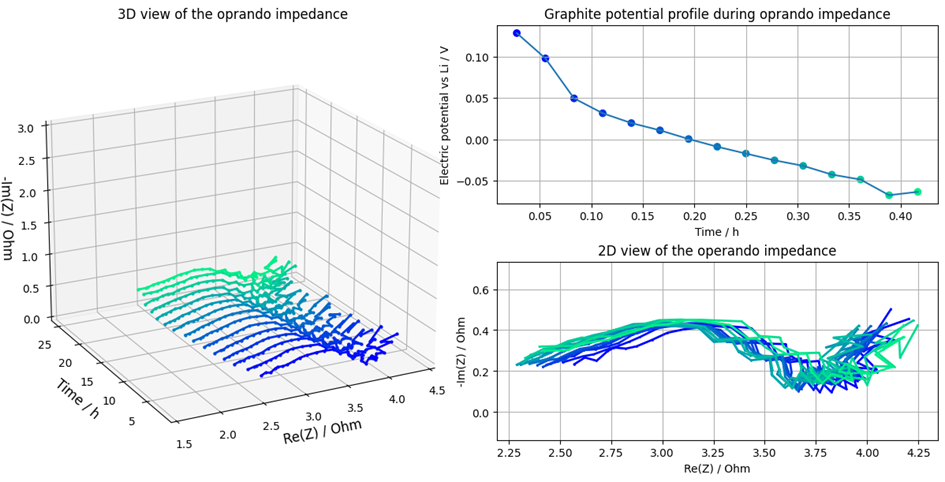
\includegraphics[width=\linewidth]{figures/application5/image5.png}
\end{figure}

\begin{figure}[H]
    \centering
    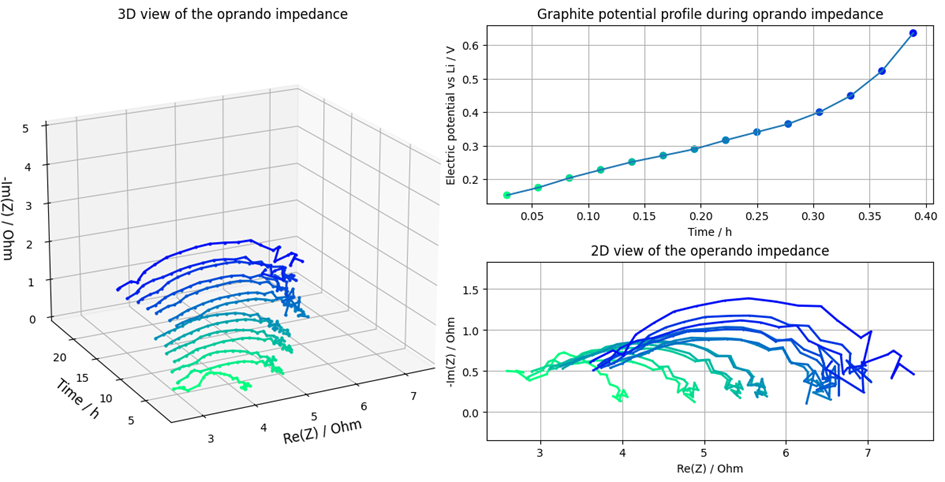
\includegraphics[width=\linewidth]{figures/application5/image6.png}
\end{figure}

\begin{figure}[H]
    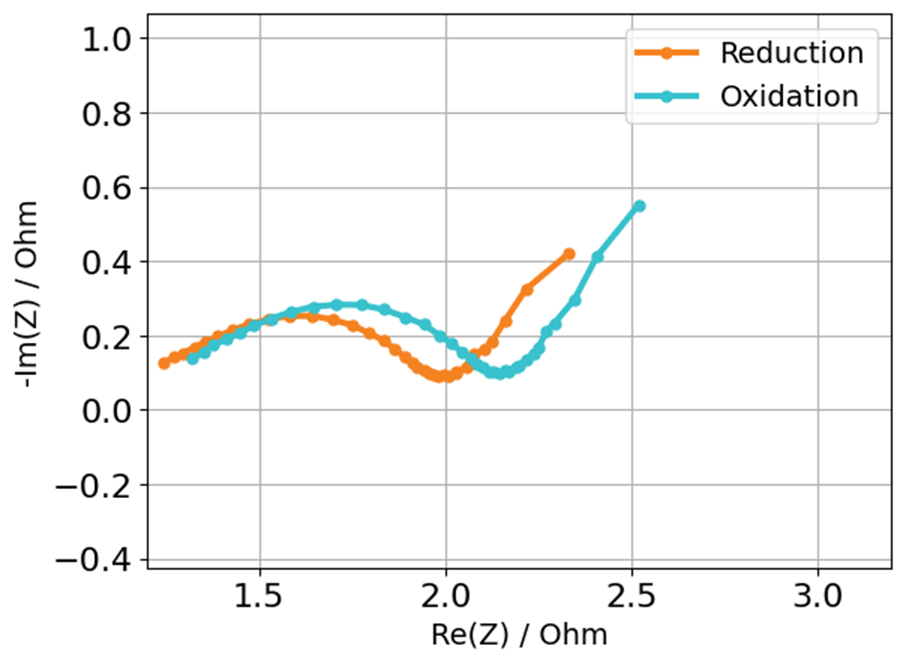
\includegraphics[width = 5cm]{figures/application5/image7.png}
\end{figure}

\begin{figure}[H]
    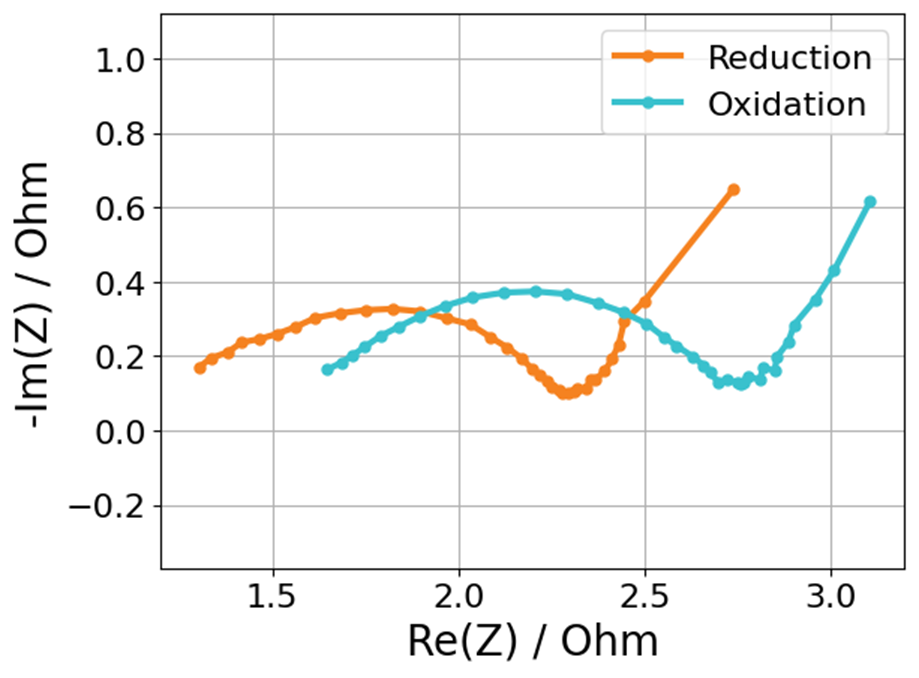
\includegraphics[width = 5cm]{figures/application5/image8.png}
\end{figure}

\begin{figure}[H]
    \centering
    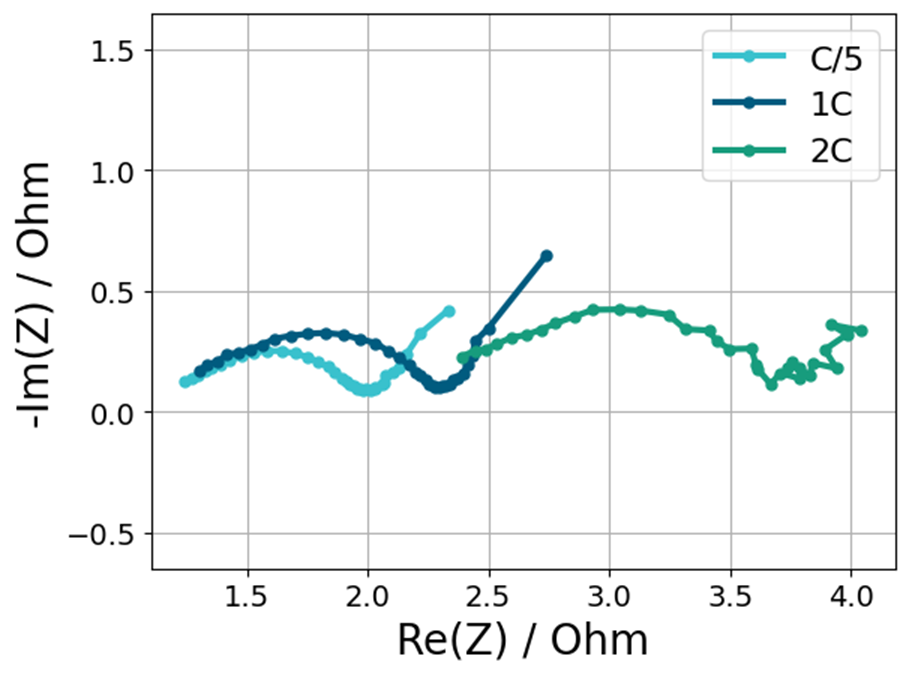
\includegraphics[width=0.7\linewidth]{figures/application5/image9.png}
\end{figure}